\documentclass[10pt,a4paper]{article}

\usepackage[utf8]{inputenc}		% Configuro la codificación
\input{config.tex}				% Archivo con los comandos globales como Título y autores
\input{preamble.tex}
\input{aux_functions.tex}		% Se proveen un conjunto de funciones extras

% Defino el path de los includegraphics
\graphicspath{{./Figuras/}}		% Directorio que contiene los graficos

% Defino el path para los input de .tex y de .eps
\makeatletter
\def\input@path{{./Figuras/}{./Secciones/}{./Cover_page/}{../Octave/graficos/}}
\makeatother

% Defino el path del listings
\ifListings
%% Cambiar el nombre de la carpeta si se utilizan Listings
	\lstinputpath{{../Octave/}}
\fi

\definecolor{myred}{rgb}{0.5,0,0}
\definecolor{mygreen}{rgb}{0,0.5,0}



\begin{document}
		% Carátula (formal o simple,_formal o _simple respectivamente) con Resumen
		% incluido e Índice (si es necesario configurar en config.tex) del informe
		\input{cover_formal.tex}
	\setcounter{page}{1}

		%\section{Polarización}\label{sec:pol}
			\begin{quote} \textit{1) Estudiar las corrientes y tensiones en todos los componentes en función del tiempo, desde que se enciende el regulador ($t=0$) hasta régimen permanente. En particular, en régimen permanente, estudiar en detalle las corrientes y tensiones en un intervalo de unos pocos periodos.}
\end{quote}

%\HgraficarPNG{0.4}{fly}{Regulador \textit{Flyback} aislado.}{fig:cto}

\begin{figure}[H]
	\centering
	\includegraphics[scale=0.5]{Figuras/1_esquematico.pdf}
	\caption{Circuito bajo análisis con \textit{PSpice}.}
	\label{fig:esq}
\end{figure}


\Flor{Simulación hecha con $Vimax = \sqrt{2} 220V = 311V$. }
\begin{figure}[H]
	\centering
	\includegraphics[scale=0.5]{Figuras/1_transitorio_con_rectificador.pdf}
	\caption{Transitorio.}
	\label{fig:transitorio}
\end{figure}

\begin{figure}[H]
	\centering
	\includegraphics[scale=0.5]{Figuras/1_regimen_permanente.pdf}
	\caption{Régimen permanente.}
	\label{fig:permanente}
\end{figure}



		%\section{Variación de la carga}\label{sec:variacion_carga}
			\begin{quote} \textit{2) Luego de haber estudiado como está operando el circuito con las cargas $R_1$ y $R_2$ en su valor de diseño (\SI{6}{\ohm} y\SI{1.25}{\ohm} respectivamente), estudiar cómo opera el circuito si éstas varían hacia valores mayores y menores.}
\end{quote}

		%\section{Estudio de componentes}\label{sec:componentes}
			\begin{quote} \textit{3) En base al estudio del ítem anterior verificar si los semiconductores sobrevivirán el estrés del régimen transitorio y la operación en régimen permanente. O sea, determinar si los semiconductores $M_1$, $D_1$ a $D_7$ son adecuados para este diseño, justificar y en caso de que alguno o algunos no lo sean, encontrar un sustituto que sí. Justificar este estudio en las características publicadas por los fabricantes de los semiconductores. }
\end{quote}

		%\section{Variación del ciclo de trabajo}\label{sec:duty_cycle}
			\begin{quote} \textit{ 4) El regulador se ha diseñado para operar en modo discontinuo con $D<0,5$. Verificar si para $D>0,5$ el regulador pasa a operar en modo continuo. ¿Qué observará en las señales de tensión y corriente de todos o alguno de los componentes para determinar el si el regulador está operando en modo continuo o discontinuo?}
\end{quote}

%\Flor{ Creo que falta algún gráfico, mepa que no pusheaste las simulaciones Nico} 
	Se cambio el valor del ciclo de trabajo a  $ D= 0,8 $ y se obtienen los siguientes resultados

\begin{figure}[H]
	\centering
	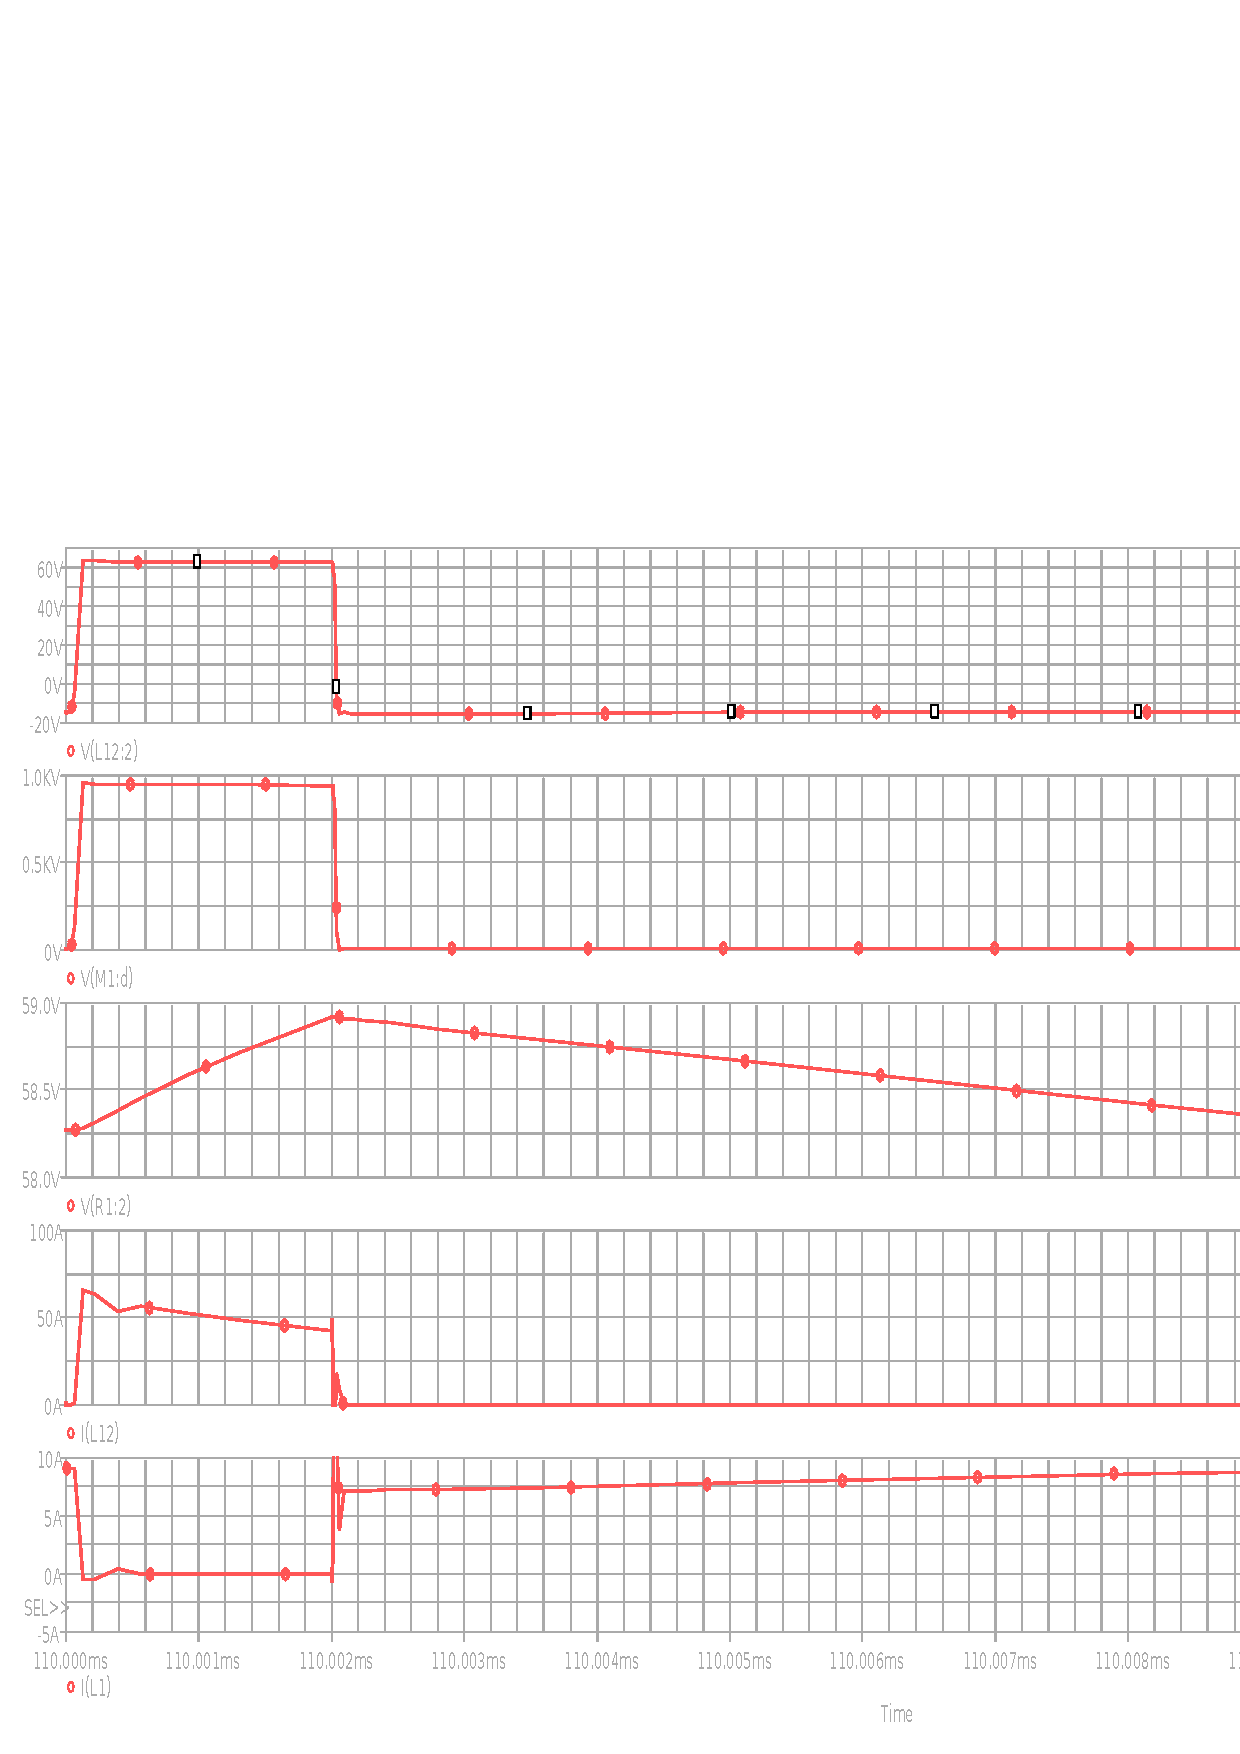
\includegraphics[width=\textwidth]{Figuras/ej4_sim.pdf}
	\caption{Régimen permanente en modo contínuo.}
	\label{fig:permanente_mcc}
\end{figure}

	Como se puede observar en \ref{fig:permanente_mcc} el circuito superado el ciclo de trabajo máximo pasa a operar en modo contínuo, ya que la corriente en el inductor no se interrumpe en todo el ciclo de trabajo. 
	\indent En el caso de que se quiera seguir operando en modo discontínuo para dicho ciclo de trabajo se deberia utilizar los siguientes valores de inducciones. 

\begin{align*}
	\centering
	& I_{max} = \frac{ 2 \cdot \SI{36.4}{\watt} }{\SI{150}{\volt} \cdot \num{0,8}} = \SI{0.61}{\ampere} \\
	& L_{1,max} = \frac{\SI{150}{\volt} \cdot \num{0,8}}{\SI{0.61}{\ampere} \SI{100}{\kilo\ohm}} \simeq \SI{1.97}{\milli\henry} \\
	& N_{12} = \frac{ (12+1)(1-0,8) \cdot N_1}{ (150-2) \cdot 0,8} = \frac{13 \cdot N_1}{592} \implies \boxed{L_{12} \simeq \SI{0.95}{\micro\henry}} \\
	& N_5 = \frac{(5+1)(1-0,8) \cdot N_1}{(150-2) \cdot 0,8} = \frac{3 \cdot N_1}{296} \implies \boxed{L_5 \simeq \SI{0.2}{\micro\henry}}
\end{align*}


%\begin{itemize}
%	\item Modo continuo:\hspace{0.4cm} $ \frac{1}{2} \Delta I_L < I_o $
%	\item Modo discontinuo: $ \frac{1}{2} \Delta I_L > I_o $
%\end{itemize}


%\begin{align*}
%	\centering
%	D_{max} &= 0,5 \implies \frac{1}{2} \cdot \SI{20}{\ampere} > I_o = \SI{2}{\ampere} \\
%	D_{max} &= 0,8 \implies \frac{1}{2} \cdot \SI{7.5}{\ampere} > I_o = \SI{2}{\ampere}
%\end{align*}

		%\section{Valor del capacitor}\label{sec:C3}
			\begin{quote} \textit{5) Determinar el valor adecuado de C3.}
\end{quote}


\Flor{Ecuaciones de Nico. No entendí de dónde sale el 280V. ¿No sería $\SI{220}{\volt} \sqrt{2} = \SI{311}{\volt}$?}
\begin{align}
	V_{max}  &=\SI{311}{\volt} \\
	V_{med}  & = \frac{\SI{311}{\volt}\cdot 2}{\pi} = \SI{198}{\volt} \\
	V_{ripple} &= 10\% \cdot V_{med} = \SI{19.8}{\volt}\\
	I_{med} &= \frac{V_{med}}{R_L} = \frac{\SI{19.8}{\volt}}{\SI{3}{\ohm}} = \SI{6.6}{\ampere} \\
	C_3 &= \frac{I_{med}}{V_{ripple}2f} = \frac{\SI{6.6}{\ampere}}{\SI{19.8}{\volt}2 \SI{50}{\hertz}} = \boxed{\SI{3.3}{\milli\farad}} \\
\end{align}


		%\section{Características de capacitores}\label{sec:caps}
			\begin{quote} \textit{6) Dimensionar todos los capacitores, o sea, tamaño, formato, tecnología, tolerancia, máxima potencia y/o tensión y temperatura, resistencia efectiva serie, frecuencia de operación máxima, tiempo de vida útil, etc.}
\end{quote}
\Flor{Creo que 120uF y 470uF vienen solo electroliticos, aunque son malos para alta frecuencia}
\begin{table}[H]
	\centering
	\begin{tabular}{cccccccc}
		\toprule
		& Valor & $V_{max}$ & Tipo & ESR & tol. & vida útil &f \\
		\midrule
		$C_1$ & \SI{470}{\micro\farad} & \SI{25}{\volt} & electrolítico &  & 10\% & &  \\
		$C_2$ &\SI{120}{\micro\farad} & \SI{16}{\volt} & electrolítico & & 10\% & &\\
		$C$ &\SI{3300}{\micro\farad} & \SI{250}{\volt} & electrolítico & \SI{0.4}{\ohm} & 20\% &  2000hs a \SI{105}{\celsius} & \\
		\bottomrule
	\end{tabular}
\end{table}

		%\section{Controlador}\label{sec:controlador}
			%\begin{quote} \textit{7) Se requiere que el regulador actúe en forma automática ante cambios en la carga y/o en la fuente de entrada, para lo cual es necesario diseñar un circuito controlador que sense la tensión de salida y varíe apropiadamente el ciclo de servicio D (reemplazando el generador de pulsos mostrado en el esquema presentado en esta actividad). Esto puede lograrse con un circuito auotoscilante (generalmente discreto con unos pocos transistores) o con un circuito integrado dedicado. Investigar ambas soluciones y plantear una adecuada.}
%\end{quote}


Con el fin de realizar un análisis cualitativo del circuito autosclilante en régimen permanente, se representa a la tensión entregada por el rectificador con un tensión constante $Vi$, según se indica en la Figura \ref{fig:cto_auto}. 

\begin{figure}[H]
	\centering
	\includegraphics[scale=0.4]{Figuras/auto.eps}
	\caption{Circuito autosclilante.}
	\label{fig:cto_auto}
\end{figure}


En principio en el nodo A, hay una tensión positiva, por lo que el transistor esta en conducción, por lo que circula una corriente IL. Por inducción hay una corriente de salida ya que el diodo D1 está en directa. A su vez se genera una tensión inducida en L3, inversa a la de entrada, por ende el transistor entrará en corte. \\


El controlador puede implementarse mediante el circuito integrado \texttt{TL494}, según se indica en la Figura \ref{fig:cto_tl494}. El controlador actúa como un realimentador, toma una muestra de la tensión de salida y la compara con una tensión de referencia mediante un amplificador de error. Ante una variació en la salida, cambia la tensión en el \textit{gate} del MOSFET y por ende la corriente que circula por el inductor primario. De esta manera se logra regular le ciclo de trabajo D.


\begin{figure}[H]
	\centering
	\includegraphics[scale=0.4]{Figuras/tl494.eps}
	\caption{Controlador con \texttt{TL494}.}
	\label{fig:cto_tl494}
\end{figure}


		%\section{Protección}
			\begin{quote} \textit{8) Considerar también la forma de proteger la carga, el regulador y la fuente primaria implementando los circuitos adecuados. Este último tema no es obligatorio para la presente actividad y puede omitirse. Sin embargo se recomienda tenerlo presente en todo diseño de reguladores conmutados o lineales.}
\end{quote}

Con el fin de evitar daños en la carga, se puede implementar el circuito de protección \textit{Crowbar}, el cuál consiste en anexar un tiristor, zener y fusible según se indica en la Figura \ref{fig:crowbar}. En condiciones normales de operación, los componentes agregados no alteran el funcionamiento del circuito original, sólo si la tensión de salida supera cierto umbral el tiristor se activa y el fusible se quema.


\begin{figure}[H]
	\centering
	\scalebox{0.5}{% XCircuit output "crowbar.tex" for LaTeX input from crowbar.eps
\def\putbox#1#2#3#4{\makebox[0in][l]{\makebox[#1][l]{}\raisebox{\baselineskip}[0in][0in]{\raisebox{#2}[0in][0in]{\scalebox{#3}{#4}}}}}
\def\rightbox#1{\makebox[0in][r]{#1}}
\def\centbox#1{\makebox[0in]{#1}}
\def\topbox#1{\raisebox{-0.60\baselineskip}[0in][0in]{#1}}
\def\midbox#1{\raisebox{-0.20\baselineskip}[0in][0in]{#1}}
   \scalebox{1}{
   \normalsize
   \parbox{4.5625in}{
   \includegraphics[scale=1]{crowbar}\\
   % translate x=558 y=152 scale 0.38
   \putbox{4.07in}{1.86in}{1.20}{Zener}%
   \putbox{4.07in}{1.61in}{1.20}{25V}%
   \putbox{4.07in}{1.36in}{1.20}{11V}%
   \putbox{0.44in}{2.62in}{1.20}{Fusible}%
   \putbox{2.94in}{1.93in}{1.20}{RL}%
   \putbox{1.87in}{2.23in}{1.20}{Circuito}%
   \putbox{0.70in}{1.88in}{1.20}{Tiristor}%
   \putbox{0.88in}{1.65in}{1.20}{9A}%
   \putbox{0.79in}{1.43in}{1.20}{(min)}%
   } % close 'parbox'
   } % close 'scalebox'
   \vspace{-\baselineskip} % this is not necessary, but looks better
}
	\caption{Protección por sobretensión.}
	\label{fig:crowbar}
\end{figure}



		%\section{Conclusiones}\label{sec:conclusiones}
			\input{9_conclusiones.tex}
	% \appendix
\end{document}
